\documentclass[12pt]{article}
\nonstopmode
\title{\vspace*{\fill}\Huge Lab n: Title}
\author{Ashraf Mrabet, Partner}
\date{Experiment date: MM/dd/20XX\\ Submitted on MM/dd/20XX\vspace*{\fill}}
\usepackage[a4paper, margin=1in]{geometry}
\usepackage{amsmath, amsfonts, amssymb, esint, systeme}
\usepackage{graphicx}
\usepackage{tikz}
\usepackage[american,siunitx]{circuitikz}
\usepackage{pgfplots}
\usepackage{hyperref}
\hypersetup{colorlinks = true, urlcolor = black}


\begin{document}
	
	{\Huge \maketitle}
	
	\newpage
	
	\section{Introduction}
	
	\ \ \ \ \ Our goal in this lab is to...

	(provide historcal context)$^{[1]}$
	
	\section{Theory}
	\begin{center}
		\begin{tikzpicture}
			\draw (0,0) -- (5,0) -- (5,5) -- (0,5) -- (0,0);
			\fill [gray] (0.5,2.5) circle (0.3);
			\draw [->] (0.5,2.5) -- (4.5,2.5) [green] node[below] {$c\vec{v}$};
		\end{tikzpicture}
		\begin{circuitikz}
			\draw (0,0) to [battery1, invert, v<=$V$, i>=$I$] (0,5) to [C, v=$v_C$ ,l=$C$] (5,5) to [R, l=$R$] (5,0) to [L, v=$v_L$ ,l=$L$] (0,0);
			\draw (5,1.25) to (6.5,1.25) to [rmeter, t=V, v<=$\sqrt{2}V_{R_{max}}$] (6.5,3.75) to (5,3.75);
			\ctikzset{bipoles/oscope/waveform=sin}
			\draw (5,1.25) to (3.5,1.25) to [oscope] (3.5,3.75) to (5,3.75);
		\end{circuitikz}
	\end{center}
	
	(Derive formulas to be used in analysis and the idea behind them)$^{[2]}$

	\section{Procedure}
	(explain what happened during lab)
	
	\section{Analysis}
	(Goal and results)
	
	\begin{center}
		\begin{tabular}{|c|c|}
			\hline
			quantity 1 (unit 1) & quantity 1 (unit 1)\\
			\hline
			value 1 & measurement 1\\
			value 2 & measurement 2\\
			\hline
		\end{tabular}
	\end{center}

	\begin{center}
		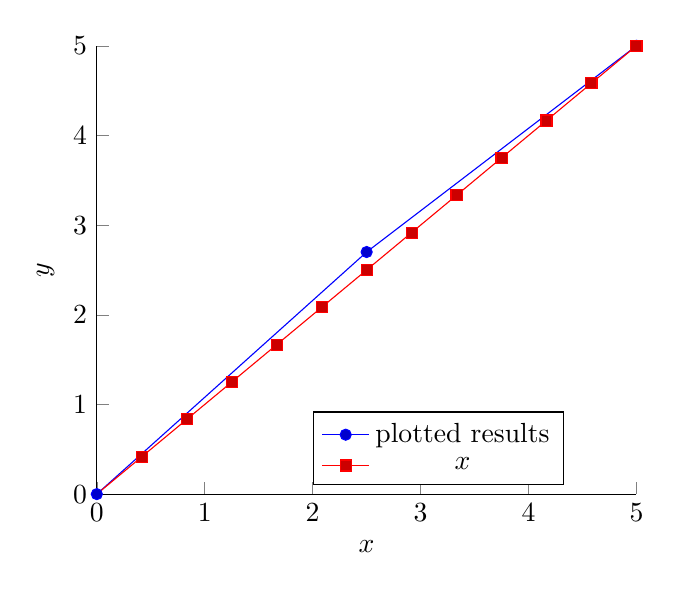
\begin{tikzpicture}
			\begin{axis}[ 
				xmin=0,xmax=5,xlabel=$x$,
				ymin=0,ymax=5,ylabel={$y$},
				axis lines*=left,scale=1,
				legend style={at={(axis cs:2,0.1)},anchor=south west}
				] 
				\addplot coordinates {
					(0,0)
					(2.5,2.7)
					(5,5)
				};
				\addplot {x};
				\legend{plotted results,$x$} 
			\end{axis}
		\end{tikzpicture}
	\end{center}
	
	(final quantities deduced and error)
	
	\section{Discussion}
	(Disucuss possible reasons for error and suggest improvements)	

	\section{Conclusion}
	...
	
	\begin{thebibliography}{}
		\bibitem {1}
		\href{URL}{Website}
		\bibitem {2}
		First M. Last (2000) \emph{Source}, page/publisher/info.		
	\end{thebibliography}
	
\end{document}
